%*******************************************************************************
%*********************************** First Chapter *****************************
%*******************************************************************************

\chapter{Introduction}  %Title of the First Chapter 
\label{chap:Intro}

\graphicspath{{Chapter1/Figures/} {Chapter1/Figures}}
\begin{quote}
%\textsl{One should never try to prove anything that is not almost obvious - Alexander Grothendieck}
\textsl{There are things known and there are things unknown, and in between are the doors of perception} - Aldous Huxley - \textsl{Doors of perception}
\end{quote}


\section{Introduction}

We live in a world where information is being bombarded on our cognitive faculties from all sides, at all times. The internet is a continuous stream of information and each source is fighting with the other to get a piece of our attention budget. 
With the advent of machine learning and big-data, building systems that predict actions as a response to perceptual triggers has become the bread and butter of many companies. The use cases may range from understanding which adverts made a visitor do an unscheduled purchase, or which string of music tracks recommendations maximized a users time on a particular music platform. But in the end it all boils down to understanding what triggers result in human action or lack there of~\cite{song2012survey}. Nonetheless the systems that surrounds a human interacting with the internet, are all figuring out the best triggers which are perceived by the human as worthy of attention. 
The term ``Attention Economy''~\cite{davenport2001attention} was actually coined for this very reason. In the words of Matthew Crawford ``\textit{Attention is a resource, a person has only so much of it.}''~\cite{MatthewCrawford}. We live in the age of distraction, and more often than not our subjective perceptions are guiding our actions, instead of our conscious cognitive processes. Several studies have shown that engagement is almost always a game of stimulating our most basic urges, such as dopamine hits, presence of faces or simply arousal of emotions to increase the working memory.~\cite{bakhshi2014faces,joglekar2017like}~\cite{schupp2006emotion}~\cite{soat2015social}. 

On the positive side of this story, the capacity of subjective perceptions to influence actions, is also being used to design positive interventions. One such example is the emergence of more formal topical spaces on the internet, that facilitate providing peer-to-peer perceived social support~\cite{coulson2005receiving,balasooriya2016barriers} or information exchange~\cite{frost2008social}. The ever pervasive nature of the internet allow these formal spaces to function almost like physical communities, with moderated and effective peer to peer exchange of thoughts, ideas and empathy~\cite{kummervold2002social,squire2015should,hwang2010social}.

There has also been a series of works~\cite{jang2019crowd,quercia2014aesthetic,quercia2015smelly,quercia2015chatty,quercia2014shortest} that looked into whether we can quantify the perception of the physical world based on the crowd-like behaviour of individuals online. Here crowd-like implies that there is no social interaction between two individuals generating the interaction data. These individuals take actions online(check-in on a platform, post a picture, tweet etc) influenced by their perceptions of the real physical space. In these situations, their perception of real spaces is influencing what they post, like, do online.
 
Both these examples show that in the age of the internet, our online and offline lives have been linked more deeply than ever. Our once assumed offline personal needs, like social support,  are being addressed via online forums. At the same time, actions that we take offline are enriching and influencing our online presence. In both cases the subjective perception of our online and offline environment is impacting or life experience. This provokes the question:

\noindent\fbox{\begin{minipage}[t][2\height][c]{\dimexpr\textwidth-2\fboxsep-2\fboxrule\relax}
        \label{guiding_principle}
        \centering
        Can quantifying the interactions that are driven by our subjective perceptions, help us design impactful interventions for our on-line and offline lives? 
%        
\end{minipage}}

\vspace{1cm}
%These two questions are going to be the guiding principles of my dissertation.
This question has been the guiding principle of my dissertation. 
But first, we need to clarify the framework that grounds this dissertation's approach towards perception, affect and data. To do so we should try and understand each of these terms separately. 


\section{Perception and Affect}
In this dissertation, I tried to build frameworks to capture the signatures of perception of the subjective. This was accomplished using large volumes of data and metrics designed around concepts from inter disciplinary fields. The utility of such an attempt, can only be justified if there is a real link between how humans take decisions at the most fundamental cognitive level and how they perceive the world around them. If there exists such a link, then the signatures found in the data can be explained and capitalized. 

There has been an ongoing effort to unravel this link, through psychological, neuro-evolutional and philosophical arguments. I will try to gain inspiration from them, but a detailed critique is beyond the scope of my dissertation and expertise\\
\begin{definition}
    \textbf{Affect~\footnote{American Psychological Association definition.}}: Any experience of feeling or emotion, ranging from suffering to elation, from the simplest to the most complex sensations of feeling, and from the most normal to the most pathological emotional reactions.\\
\end{definition}


\begin{definition}
    \textbf{Perception~\footnote{American Psychological Association definition.}}: The process or result of becoming aware of objects, relationships, and events by means of the senses, which includes such activities as recognizing, observing, and discriminating. These activities enable organisms to organize and interpret the stimuli received into meaningful knowledge and to act in a coordinated manner.
\end{definition}


Emotions or `affects' and perceptions have long been discussed in the psychology, neuroscience and philosophical literature. The two are tightly linked in our understanding of mind. Perception is a process, and affect is a result that this process sometimes evokes.  
Emanuel Kant in his prolific work, first discussed the utility and the philosophical reasoning behind presence of affects or emotions\cite{kant1987critique}. In his opinion, emotions are pre-cognitive involuntary states, termed as "mere perceptions of unspecified bodily states"\cite{borges2004can}. 
But according to him, that does not mean they don't influence our deepest level of well-being and decision making processes.
The link between affect and perception has also been explored in several other cases. One way to look at it was through the framework of understanding the aesthetic. In some sense, the aesthetic is an affect inducing entity. The act of enjoying a gorgeous sunset or a beautiful flower defines a sentient perceptive mind, as much as language or art.  
An argument to link the aesthetic with perceptions was made by Perlovsky\cite{perlovsky2014aesthetic}, where they propose that the phenomenon of affects arousing from perception of aesthetics, comes from a fundamental human need to enrich the knowledge about real world. An unexpected thing, stimuli or structure in physical space creates a dissonance between our expected model of the world and the perceived reality. And at some level we perceive it as aesthetically pleasing. Another recent study by Zadra et.al\cite{zadra2011emotion} evaluated the relation between visual perception and emotions. They demonstrate that the conventional assumption of the disentangled functioning of perception and affects is not true. Humans are quite susceptible to perceiving different realities based on different aroused affects. So a happy person would perceive a 50\$ shoe to be a reasonably priced item, which a sad person may not. 

The discussion on the formal definition and process of affects will continue, but there seems to be a consensus, at-least among the computer science and information science community that affects do influence our decisions and we perceive information through a filter of affects. Affective triggers can be generated when information is formatted or packaged in a certain way. 

In such a setup, it is worth testing if certain affect driven interactions on the web leave a trail of patterns in the data of these interactions. Furthermore it is worth asking if these patterns might in some way be used to improve, through interventions, our online and physical environments. But to arrive at these patterns, one needs to formalize the frameworks for approaching such a problem. 
The journey from Data to the subjective signatures needs to be standardised. 

\section{The DIKW model}

\begin{figure*}[t!]
    \centering
    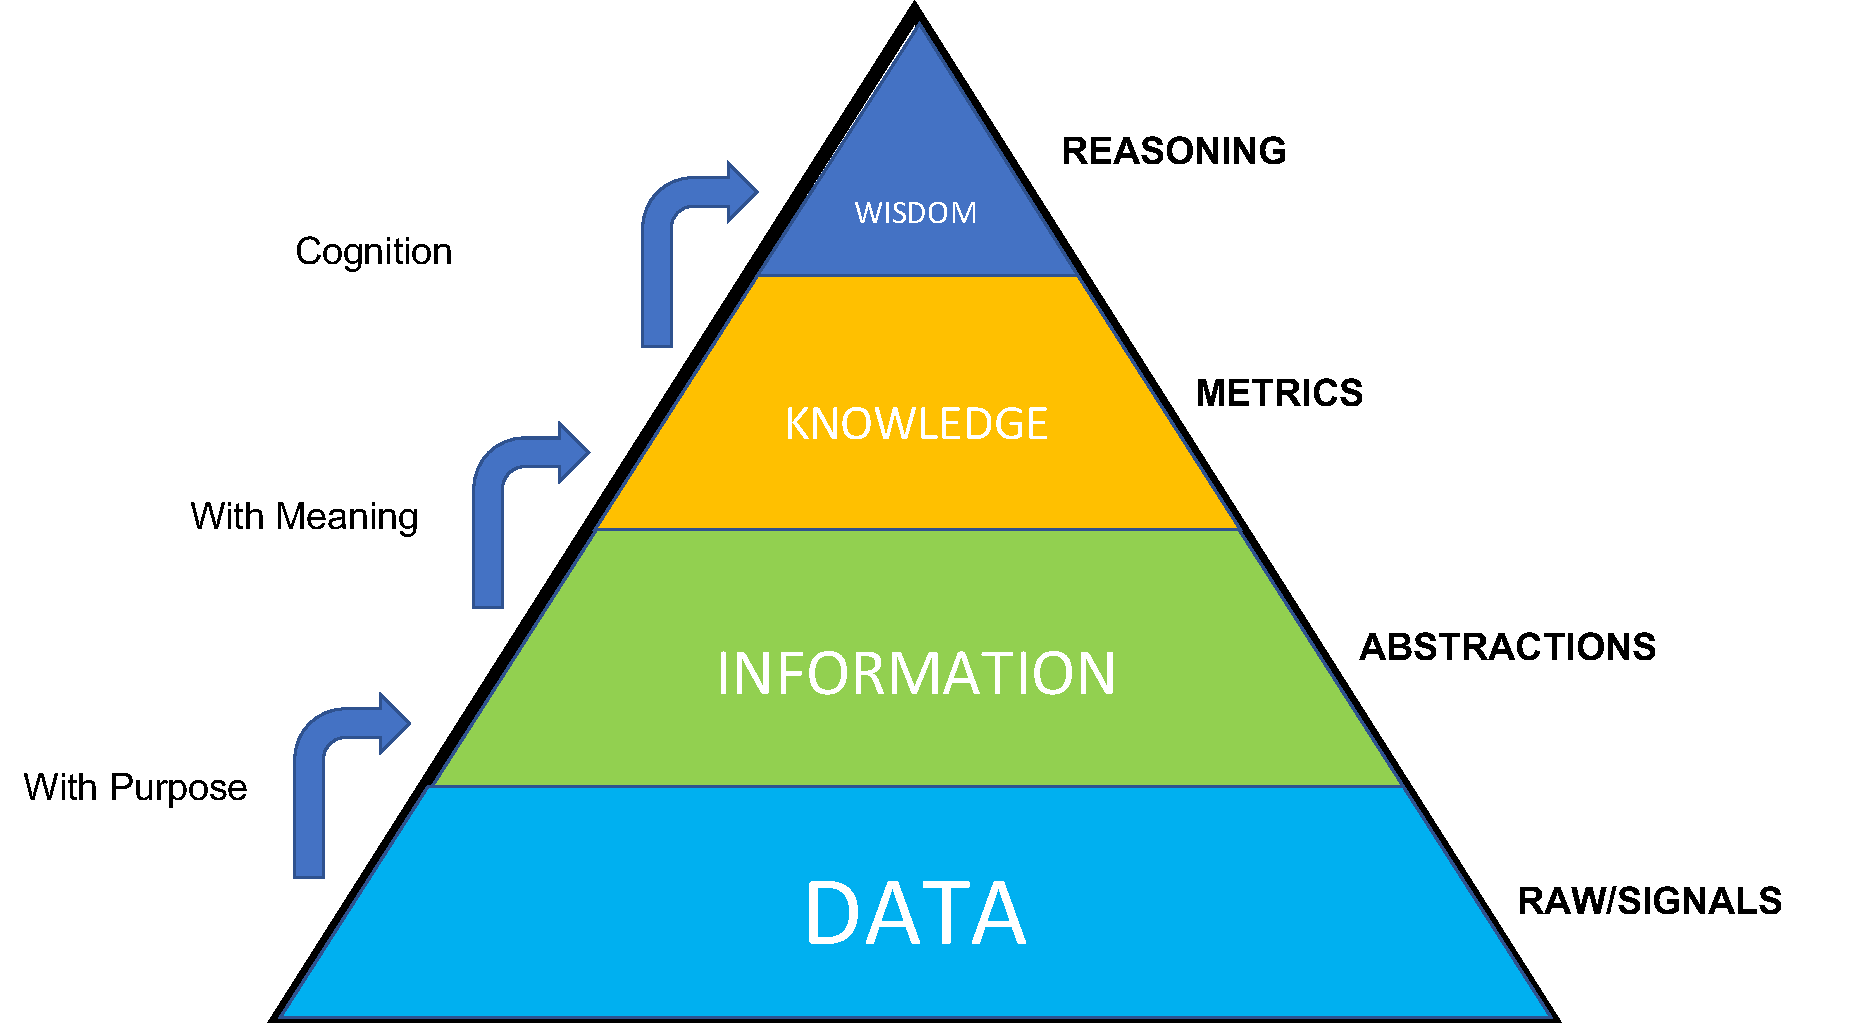
\includegraphics[width=\columnwidth]{DIKW.pdf}
    \caption{The DIKW pyramid}
    \label{fig:dikw}
\end{figure*}

On the journey to develop metrics and pipelines, one has to reflect on frameworks that codify operations on data. One such framework, which I found relevant to my work, is the \textbf{Data , Information, Knowledge and Wisdom} model~\cite{rowley2007wisdom}. In this dissertation I posit and demonstrate through case studies, that for any reasoning about subjective perceptions, we need to develop frameworks that extract knowledge from data in a format that is aligned with the ontological framework of the application. In the context of this dissertation, ontology implies a set of concepts, definitions and relations between entities defined around a common set of axioms. I use these ontological constructs to derive meaning from the metrics I design. 

But this framework follows a pyramidal framework where with each layer the data gains more structure and the relationships become more defined. In this model, the most foundational layer consists of the pure form raw \textbf{Data or signals} that come from a source. If we are measuring subjective perceptions of humans, this source needs to be tied back to humans in some way. To that extent, the data must ideally be a product of human to human interaction online. Or it needs to capture the human perceived responses, through explicit exercises like crowd sourcing or public surveys. In this dissertation, I present solutions in the context of exactly these use cases, where the data sources are either from human to human interactions or a result of crowd based perception. 

The \textbf{Information} layer compels any processing done on the data, to be with a sense of purpose or an end goal. For example, if the goal is to understand how humans exchange messages at times of distress, you would most certainly need to express the raw information about sender and recipient of messages into some form of a networked abstraction. This compulsion of goal generally forces us to choose an abstraction to structure the data into. The abstraction preserves the organization of data, but at the same time allows information to be operated on.  

\textbf{Knowledge}. Defining knowledge has been an ongoing effort in the field of philosophy. But in the context of information science, knowledge involves collation of diverse sources of information and mix of contextual information, values and metrics to deliver a coherent understanding of the real world. For example, if you need to know the most popular user among a social network of users exchanging messages; you would look for the most central user in the network(abstraction) along with several other temporal and structural metrics to arrive at a few candidates. In this particular case, these metrics, along with the context of the social network's design, dawns the meaning of ``popularity''. 

The final layer needs a cognitive process and an ontological framework, to extract actionable insights which we can call \textbf{wisdom}. The classical definition of ontology defines it as properties of and relations between objects or concepts. For this very reason, these ontological frameworks need to originate from the fields of intervention.  In our example, let's assume we need to get some insights about the dynamics of popular users. Particularly in the context of optimizing advertising delivery. For example we need to understand how a particular piece of advertising might percolate through the network if certain popular users advertise it~\cite{li2012diffusion}. However , to arrive at these insights we need to be grounded in the ontological frameworks of epidemiology, network physics and depending on the application, advertising or meme theory. Then using the abstractions of social networks, the metrics derived from them, and the ontological basis of all the aforementioned fields, one can design a pipeline that could deliver us these insights with reasonable accuracy. This pyramidal approach inspires all the frameworks and data processing pipelines I developed in this dissertation. Figure \ref{fig:dikw} shows an illustration of the adopted version of Rowley's DIKW model, which I would refer back as a repeating motif throughout my dissertation.

\subsection{Data}
Data is one of the most fundamental contribution of this work. To develop frameworks around quantification of human perceptions, so that we can do impactful interventions from this approach, we first need to make sure we formalize how we acquire, clean and condition our data. The base level of this pyramid is the data that the framework would work with, in order to ascend to extract the wisdom. I worked with diverse forms of data such as textual data , video data and image data to understand how these might exhibit signatures of human perceptive processes. The relation between data and subjective attributes needs to be examined using some proxy. For this reason, my research involved collecting data from sources where either human to human interactions happen, or the data is generated on account of a human expressing their opinion about a subjective quality, like in case of crowd based perceptions.

\subsubsection{Interaction Data}
The first case study of this dissertation focuses on online support communities, where human to human interaction is at the centre of these communities. It has been shown through several studies in medical informatics, that these communities play a very important role in providing support and respite in times of distress~\cite{allen2016long}~\cite{mo2012developing,pendry2015individual} ~\cite{bartlett2011investigation,izuka2017stroke}~\cite{hobbs2016online}. The communities are especially helpful when it comes to people suffering from long term illnesses or mental health issues.
The key element that impacts the users is the perceived social support~\cite{nambisan2011information}, which delivers people in distress a sense of belonging to a group and empathy from the fellow supporters. 
To understand how users on these communities perceive social support, I work with data acquired from online health forums, where users share, give support and ask for support. I look at communities that deal with long term conditions like Lung illnesses, and communities where mental health patients seek support~\cite{joglekar2018online}. The data spans across a duration of 10 years, containing peer to peer support interactions of more than 30,000 users. I also crawled a popular forum based social network called reddit \footnote{\url{www.reddit.com}} to acquire a peer to peer support data regarding mental illness and suicidal thoughts. The data covers discussions around  more than 30,000 calls for support, and includes the complete structure of the way people respond to these calls. 

\subsubsection{Image data}
The other facet of my work looks at the problem of quantifying our perception of physical spaces. Whether a street is considered beautiful is a matter of subjective opinion. And yet research has shown that there are specific urban elements that are universally considered beautiful: from greenery, to small streets, to memorable spaces~\cite{alexander1977pattern, quercia2014aesthetic,salesses2013collaborative}. These elements are those that contribute to the creation of what the urban sociologist Jane Jacobs called `urban vitality'~\cite{jacobs1961death}. Apart from vitality, these motifs in urban environments are also highly correlated with feeling of well-being, health and safety~\cite{kaplan1989experience}. There have been studies where people have tried to use crowd sourcing to acquire subjective ratings of images~\cite{seresinhe2015quantifying} which have shown some reasonable progress on this front. But the real gap in these studies is understanding the impact of urban elements on the perception of these subjective qualities. E.g. How much does presence of a green garden affect the subjective rating of beauty for that particular area? For this reason, I work with google street view data and crowd sourced subjective ratings of various places around the world~\cite{naik2014streetscore}, with the aim to understand how people perceive the sense of beauty in urban areas. Then using the ontological basis of urban design and architecture, developed by a detailed literature review, I aim to develop machine learning pipelines that can suggest interventions to change perceptions of physical spaces.

\subsection{Abstractions}
The act of aggregating information from data, almost always involves building structured abstractions. Throughout my dissertation, I either repurpose well known abstractions in computer science or develop my own using tools from fields like computer vision and Information theory. For the first study, I incorporate user meta data and the textual data of their activity, to build organized networked abstractions representing the conversation structures on the support forums. I use these abstractions to evaluate global and local structures in support communities, which would be discussed in detail in Chapter \ref{chap:Utility_support} and \ref{chap:structure_support}. 
  
While working with image data, I use several pixel level abstractions to segment and group semantically similar pixels. I also use several state of the art object and scene detection algorithms, to extract semantic information from an image, with the aim at analysing correlations with the perception of subjective attributes of images with these metrics. I also use deep convolutional networks and generative models, to abstract out a representation of beauty. There will be a more detailed discussion of these abstractions in the later chapters (Chapter \ref{chap:quant_perception} , Chapter ~\ref{chap:generation}).  

\subsection{Knowledge}
For extracting knowledge, we need to first associate meanings to certain computable metrics that we obtain from the abstractions. As discussed in the previous example, it could be as simple as associating the property of ``popularity'' to the metric of centrality. In my case, I develop several of these metrics to related subjective properties with measurable structures in data. Some of these metrics are based on intuitions which I validate, and some based on extensive literature survey. To give an example, I develop the concept of anchored triads, which combines local structures in interaction graphs of users, with the role of a user in a supportive conversation. This helps me to understand how these conversations evolve.

\subsection{Wisdom}
Finally the wisdom , in definition underlies insights that come for experience. The experience could come simply from the scale of data or from cross disciplinary literature that puts forth theories of subjective experience. E.g. The theory of social support puts forth four categories of social support 1)Affective/Perceived 2)Instrumental 3)Informational 4)Networked~\cite{cutrona1992controllability}. Each type has its own specific traits. My dissertation looks at these theories from the lens of computational social science and networks science to develop metrics and methods to partly quantify signatures social support.

\section{Research Thesis and Research Questions}
To make any progress towards answering the guiding principle as articulated in \ref{guiding_principle}, we first need to make progress towards quantifying the subjective.
Hence the overarching thesis of interest that I would explore through the two case studies is:

\vspace{0.5cm}
\noindent\fbox{\begin{minipage}[t][2\height][c]{\dimexpr\textwidth-2\fboxsep-2\fboxrule\relax}		
        \label{thesis}
        How do we quantify perceived qualities from data, if the data source is human and the scale is large?    
\end{minipage}}
\vspace{0.5cm} 

But this thesis question is quite open ended, and answering it in a generalized manner seems impractical in the scope of one Ph.D. For this reason, I need to first contextualize my work in the realm  of practical applications, by deriving more focussed research questions, such that I can acquire data and test my hypothesis in an effective time bound manner. More so, to drive maximum impact, I would like to focus on applications which have the potential to have real world consequences, either through interventions or through inspired interest in the field.

\subsection{PART 1 : Supportive interactions on web communities}
Humans are social animals in every aspect. The presence of social support systems in ones lives have shown to have huge quantifiable benefits. From speeding up recovery in cases of post-partum depression or in the cases of cancer survivors~\cite{collins1993social,dunkel1984social,baron1990social} , to signs of positive turn around among patients suffering from alcoholism and depression~\cite{peirce2000longitudinal,brown1986social}, social support is a key predictor of positive prognosis for patients under distress. With the advent of internet, a lot of communities have sprung up, which provide a rich platform for patients to interact, exchange support as well as provide a perceived sense of community. These communities are moderated, only to an extent to curb toxic behaviour, but other than that are largely free form. Due to a very homogenous membership, where most members have either gone through or are going though similar distress, there is an emergent sense of support and affective empathy~\cite{de2016stroke}. The key idea of this case study was \textbf{to quantify the signatures of perceived social support in interaction patterns of these supportive communities} 

Social support, or perception of help received from others, is a widely studied as a psychological resource used to cope with distress. The social support is generally classified into one of the following categories viz. Informational, Tangible , Network or Emotional(affective)~\cite{cutrona1992controllability}. These categories measure the nature of social support along the idea of exchange of resources between the person in distress and the one providing support. For example, an informational support interaction could involve pure exchange of valuable information about dealing with an issue. Whereas as network support interaction could purely allow the recipient to acquire a wider network of people.
In the part 1 of my thesis, I would like to quantify the nature of perceived social support from the structure of the dialogue and interactions between people. I conjecture that in doing so, we can tease out the signatures of network and informational support in online communities. 
 
Quantifying these signatures would facilitate these communities to be better poised to tackle any disturbances in the dynamics of social support. These signatures would also help us quantify the net utility these communities in terms of delivered informational or network support. Hence to investigate these, I formulate the following research questions.

\noindent\fbox{\begin{minipage}[t][2\height][c]{\dimexpr\textwidth-2\fboxsep-2\fboxrule\relax}
        \label{rq1}\textbf{RQ1} \textsl{How do support communities thrive?}   
\end{minipage}}

\noindent\fbox{\begin{minipage}[t][2\height][c]{\dimexpr\textwidth-2\fboxsep-2\fboxrule\relax}
        \label{rq2}\textbf{RQ2} \textsl{How can we quantify social support on these communities?}   
\end{minipage}}
\noindent\fbox{\begin{minipage}[t][2\height][c]{\dimexpr\textwidth-2\fboxsep-2\fboxrule\relax}
        \label{rq3}\textbf{RQ3} \textsl{Are there any macro scale signatures of supportive conversations?}   
\end{minipage}}
\noindent\fbox{\begin{minipage}[t][2\height][c]{\dimexpr\textwidth-2\fboxsep-2\fboxrule\relax}
        \label{rq4}\textbf{RQ4} \textsl{Are there any meso scale signatures of supportive conversations?}   
\end{minipage}}
\vspace{1cm}

I first had to collect data from two different communities designed for online social support. The first community is dedicated for patients suffering from chronic lung diseases, such as Asthma or Chronic Obstructive Pulmonary Disorder (COPD). This community was moderated by self appointed moderators, and everyone on this community was either a survivor or a patient of these diseases. This community allowed patients to ask questions about symptoms and home remedies and sometimes just bond over social interactions. The second community I worked with dealt with people suffering from chronic depression and suicidal thoughts. This community was a safe haven for such people to vent out suicidal thoughts and get support from peers to manage these sudden flares of thoughts of self harm. 

Through these two communities, I develop a pipeline to analyse the peer to peer interactions using abstractions derived from network science. The abstractions try to mimic the conversation structure which allows me to probe the evolution of such conversations both in terms of macroscopic properties (overall structure of the network) as well as local interactions between users(mesoscopic properties). I also develop metrics inspired from psychology and sociology literature to quantify how these interactions can be qualified as supportive or non supportive. Through a data driven analysis, I establish confidence on these metrics. Through this process, I also report my findings about the dynamics of users on these communities and key properties of user roles. I find that these conversations have a distinct nature when compared against regular baseline conversations over the web, and these distinct signatures could one day be used to curb toxicity as well as improve the support community interface.

\subsection{PART 2 : Leveraging crowd's aesthetic perceptions of real spaces}
Urban aesthetics and presence of certain elements in the physical spaces that we use, have shown to have lasting effects on our mental health\cite{seresinhe2017using} and physical well being\cite{ball2001perceived,giles2005increasing}. However, with the advent of large scale data access, and machine learning techniques, we have a unique opportunity to quantify what exactly comprises of urban aesthetics.
In the next part of my dissertation, I aim at using the scale of the internet to try and improve how our cities are perceived. In this study, I investigate the following research question: 


\noindent\fbox{\begin{minipage}[t][2\height][c]{\dimexpr\textwidth-2\fboxsep-2\fboxrule\relax}
        \textbf{RQ5} \textsl{Can crowdsourcing and machine learning help us quantify how humans perceive beauty in urban settings?}   
\end{minipage}}

\noindent\fbox{\begin{minipage}[t][2\height][c]{\dimexpr\textwidth-2\fboxsep-2\fboxrule\relax}
        \textbf{RQ6} \textsl{Can we leverage the  quantification of the crowd's subjective perception, to improve real spaces?}   
\end{minipage}}

\noindent\fbox{\begin{minipage}[t][2\height][c]{\dimexpr\textwidth-2\fboxsep-2\fboxrule\relax}
        \textbf{RQ7} \textsl{Do humans and experts find the improvement realistic?}   
\end{minipage}}
\vspace{0.5cm}

Crowdsourcing is a method through which one could get inputs, subjective or otherwise, about a particular set of questions from a large number of real humans using the internet. In return the participants could be offered a tangible compensation, or in some cases, a gamified incentive. 
The \textbf{RQ5} motivates me to investigate if we can use crowdsourcing to quantify how people perceive urban spaces. Research has shown that if a large number of people could vote on a set of images, regarding their aesthetic quality, a trend emerges that favours some objective metrics of beauty\cite{datta2008algorithmic,quercia2014aesthetic}. Can we link these metrics to urban elements? For this reason we work with google streetview images, where real people vote on aesthetic value of images through a large scale crowdsourced study. After evaluating for statistical trends in preference of aesthetic urban images amongst the voters, we answer \textbf{RQ5} by training a deep convolutional neural network model, which can discern between an aesthetically pleasing and unpleasant urban scene with a high degree of accuracy. Once we have a model that could ``detect'' beauty in urban scences, we could then use machine learning and deep learning techniques to understand how different urban elements relate to the notion of beauty (\textbf{RQ6}). I further try to build a tool, which could use the quantified notion of beauty in urban spaces, to hint practitioners about possible actions to beautify any given urban space. These hints are given in the form of suggested changes in different popular urban design metrics, which makes the whole process legible to practitioners in the field. In the pursuit of answering the \textbf{RQ6} and  \textbf{RQ7}, I propose deep neural network and generative adversarial network models to make an end-to-end pipeline which can be then used to visualize how different urban elements affect the perception of beauty in the real world.

\section{List of peer reviewed publications}

I would like to list all the publications which resulted from the past 4 years of work, as well as collaborations I was able to strike with a diverse group of researchers. The author lead publications have influenced different chapters of this dissertation.

\subsection{Original author contributions}
List of papers (published, accepted and under peer review) which were either led by the author or where the author had a fundamental contribution

\begin{enumerate}
    \item \label{vinePaper} \textbf{Joglekar S}, Sastry N, Redi M. Like at first sight: understanding user engagement with the world of microvideos. In International Conference on Social Informatics 2017 Sep 13 (pp. 237-256). Springer, Cham.
    
    \item \label{JMIR} \textbf{Joglekar S}, Sastry N, Coulson NS, Taylor SJ, Patel A, Duschinsky R, Anand A, Evans MJ, Griffiths CJ, Sheikh A, Panzarasa P. How online communities of people with long-term conditions function and evolve: Network analysis of the structure and dynamics of the asthma UK and British lung foundation online communities. Journal of medical Internet research. 2018;20(7):e238.
    
    \item \label{SREP} \textbf{Joglekar S}, Velupillai S, Dutta R , Sastry N "Online discussions about mental health in Reddit exhibit signatures of supportive conversations" Under Review
    
    \item \label{RSOS} \textbf{Joglekar, S}, Redi M, Kauer T, Quercia D, Aiello L , Sastry N "FaceLift: A transparent deep learning framework to beautify urban scenes" Under Review
    
    \item \label{IEEE} Kauer T, \textbf{Joglekar S}, Redi M, Aiello LM, Quercia D. Mapping and Visualizing Deep-Learning Urban Beautification. IEEE computer graphics and applications. 2018 Sep 27;38(5):70-83..
    
\end{enumerate}

\subsection{Collaborative author contributions}
List of papers where the contribution was significant, but were not led by the author. Contributions from these articles are not included in this dissertation

\begin{enumerate}
    \item Bhatt S, \textbf{Joglekar S}, Bano S, Sastry N. Illuminating an ecosystem of partisan websites. In Companion Proceedings of the The Web Conference 2018 2018 Apr 23 (pp. 545-554). International World Wide Web Conferences Steering Committee.
    
    \item Raman A, \textbf{Joglekar S}, De Cristofaro E, Sastry N, Tyson G. Challenges in the Decentralised Web: The Mastodon Case. arXiv preprint arXiv:1909.05801. 2019 Sep 12.
    
    \item De Simoni A, \textbf{Joglekar S}, Taylor SJ, Patel A, Duschinsky R, Coulson N, Griffiths C, Panzarasa P, Sastry N, Anand A, Evans MJ. Structure and dynamics of online patients’ communities: the case of Asthma UK and BLF online fora..
    
    \item Young AP, \textbf{Joglekar S}, Garimella K, Sastry N. Approximations to Truth in Online Comment Networks.
    
    \item Boschi G, Young AP, \textbf{Joglekar S}, Cammarota C, Sastry N. Having the Last Word: Understanding How to Sample Discussions Online. arXiv preprint arXiv:1906.04148. 2019 Jun 10.
    
    \item Magdy W, Elkhatib Y, Tyson G, \textbf{Joglekar S}, Sastry N. Fake it till you make it: Fishing for Catfishes. In Proceedings of the 2017 IEEE/ACM International Conference on Advances in Social Networks Analysis and Mining 2017 2017 Jul 31 (pp. 497-504). ACM.    
   
\end{enumerate}


\section{Thesis overview}
We begin with my first case study on Online communities.
In Chapter 2 (based on article ~\ref{JMIR}), I examine how supportive communities evolve and sustain over a long period of time. I show presence of an anti-rich club effect on these support groups, which implies that experienced users are more interested in helping new comers rather than forming a clique of their own. I define a quantitative metric for ``expertise'' and show that as one becomes adept, one becomes more willing to help. All these insights point towards answers for \textbf{RQ1} and \textbf{RQ2}. In Chapter 3 (based on article ~\ref{SREP}), I look at global(macro-) and local(meso-) structures of supportive conversations. I show that mapping the conversational exchanges onto a topological structure, exhibits keen preference for local supportive motifs, which I call ``anchored motifs''. I discuss the utility of such a model of support conversation and draw parallels with the offline model of community support(Chapter 4) as per the mandate of \textbf{RQ3} and \textbf{RQ4}. 

In the second study, I investigate utility of perceptions of real world places through a crowd sourced rating of google street view images. As per \textbf{RQ5}, I develop models to extract the perception of the crowds using data driven inference methods(Chapter 4)(based on article ~\ref{RSOS}). 
I then show that a general pattern of beauty in urban spaces can be learnt through a crowd sourced opinion and based on this finding, I develop a generative model to simulate beautification of urban spaces by using deep learning(Chapter 5)(based on article ~\ref{RSOS} and article \ref{IEEE}). I validate the quantification of perception of real-world beauty using crowd validation. I contribute a way to use computer vision techniques to abstract out beautification process into explainable metrics used by architects and urban planners. The final contribution is a demo web application, that allows practitioners to examine and validate the utility of such a end to end system that captures citizen perceptions for urban design. These contributions are motivated by \textbf{RQ6} and \textbf{RQ7}. 
I close by enumerating the different research problems and future directions that my work would pursue as a early career scientist(Chapter 6)








